\documentclass[12pt,twoside,a4paper]{article}
\usepackage{amsmath, amssymb, amsfonts, mathrsfs} %les plus utiles et quasi indispensables 
\usepackage{amsthm}%\usepackage[T1]{fontenc}
\usepackage{a4wide}
\usepackage[utf8]{inputenc}
\usepackage{fancyhdr} %pour les hauts et bas de page
\usepackage[francais]{babel}% donne de bonnes c\'esures  en francais
\usepackage{titlesec}%pour modifier le style des sections
\usepackage{float}%pour fixer les flottants
\usepackage{url}%pour ecrire une adresse d'un site web
\usepackage[all]{xy}%pour faire des diagrammes
\usepackage[dvips]{graphicx}
\usepackage{todonotes}
\usepackage{graphicx}
\usepackage{pgf,tikz}
\usetikzlibrary{arrows}
\usepackage{enumitem}
\usepackage[T1]{fontenc}
\usepackage{hyperref}
\usepackage{array}
\usepackage{chemfig}
\usepackage{graphics}
\usepackage{eurosym}
\usepackage{soul}
\usepackage{wasysym}
\usepackage{textcomp}
\usepackage{listings}
\usepackage{stmaryrd}



\title{TDLog : \textsc{Jelly}}
\author{\textsc{BATY L\'eo, BRUNOD-INDRIGO Luca, CAMPO Yannis,}\\ \textsc{LAURET J\'eremy, LO Emmanuel}}
\date{15/02/2019}


\begin{document}
\maketitle

\tableofcontents

\newpage%%%

L'objectif initial de ce projet \'etait de cr\'eer un jeu multi-joueur en ligne, adaptation d'un jeu de plateau cr\'e\'e l'ann\'ee derni\`ere dans le cadre du cours de d\'eveloppement durable. 

\section{Pr\'esentation du jeu}

Dans ce jeu, les joueurs incarnent chacun un pays. Ils doivent g\'erer le d\'eveloppement \'economique, social, et environemental du pays durant deux \`eres, depuis la r\'evolution industielle jusqu'\`a nos jours. Chaque \`ere se d\'ecompose en tours appel\'es g\'en\'erations, pendant lesquels les joueurs jouent simultan\'ement en construisant des b\^atiments, recherchant des technologies et concluant des accords. Le tour suivant débute une fois que tous les joueurs ont indiqué avoir fini leur tour.

\subsection{D\'eroulement d'une g\'en\'eration}
\noindent Chaque g\'en\'eration se d\'eroule en trois phases:

\begin{enumerate}
\item Phase de revenus
\item Phase principale
\item Phase \'ev\`enements
\end{enumerate}

\subsubsection{Phase de revenus}

Chaque joueur poss\`ede trois champs principaux :
\begin{itemize}
\item ses ressources stockables : UM (unit\'e mon\'etaire) et hydrocarbures.
\item sa production exc\'edentaire : UM, hydrocarbures, nourriture, pollution, d\'echets, \'electricit\'e, r\'eg\'en\'eration de l'environnement. Par exemple, une production n\'egative de nourriture indique que le joueur doit en importer afin de satisfaire les besoins de son pays.
\item l'\'etat de son d\'eveloppement : social, \'economique, et environnemental (entier entre 0 et 100).\\
\end{itemize}

Durant la phase de revenus, chaque joueur re\c coit son revenu en UM, doit importer nourriture et \'electricit\'e s'ils sont en production n\'egative, ou les exporter s'ils sont en production positive.\\
Les revenus d'hydrocarbures fonctionnent d'une mani\`ere un peu particuli\`ere. Au d\'ebut de la partie, on constitue trois piles d'hydrocarbures repr\'esentant la r\'eserve mondiale. 

Lorsque l'on produit des hydrocarbures, on en ajoute aux ressources du joueur de la mani\`ere suivante :

\begin{itemize}
\item Tant qu'une pile n'est pas vide on prend les ressources toujours dans la m\^eme pile en commen\c cant par la premi\`ere.
\item Si au d\'ebut de la phase revenus il y avait des ressources dans la pile 1, on prend 3 hydrocarbures par point de production que l'on poss\`ede et on les place dans notre r\'eserve.
\item Si au d\'ebut de la phase revenus la pile 1 \'etait vide et la pile 2 non vide, chaque point de production rapporte 2 hydrocarbures.
\item Si au d\'ebut de la phase revenus les pile 1 et 2 \'etaient vides, chaque point de production rapporte 1 hydrocarbure.
\item S'il n'y a plus de ressources dans la r\'eserve, on n'en prend pas.
\end{itemize}


\subsubsection{Phase principale}

Durant la phase principale, les joueurs effectuent des actions de mani\`ere simultan\'ee. Voici la liste des actions possibles :

\begin{itemize}
\item Construire un b\^atiment d\'ebloqu\'e. Chaque b\^atiment a un co\^ut en UM, des modificateurs au niveau de la production du joueur et de son d\'eveloppement, et un \'eventuel effet (ponctuel ou permanent).
\item Acheter une technologie d\'ebloquable. Chaque technologie d\'ebloque une ou plusieurs technologies, un ou plusieurs b\^atiments, et poss\`ede un \'eventuel effet (ponctuel ou permanent).
\item Conclure des accords d'importation ou d'exportation. Chaque accord est propos\'e ou non de mani\`ere al\'eatoire au joueur, et r\'eduit le co\^ut des importations ou permet des exportations d'une ou plusieurs ressources pendant un certain nombre de g\'en\'erations.
\end{itemize}

Chaque joueur peut effectuer autant d'actions qu'il veut, dans la limite des fonds disponibles. Cependant, il ne peut plus construire de b\^atiments d\`es qu'il a acquis une technologie, ceci simulant que la recherche met du temps \`a porter ses fruits.

\subsubsection{Phase \'ev\`enements}

A la fin de chaque g\'en\'eration, on tire al\'eatoirement un \'ev\`enement correspondant \`a l'\`ere en cours, et on l'applique \`a tous les joueurs. Les \'ev\`enements ont des effets tr\`es vari\'es d\'ependants de l'\'etat de d\'eveloppement des joueurs. Certains s'appliquent de la m\^eme mani\`ere \`a chaque joueur, et donc regardent la moyenne (ou le minimum/maximum) de chaque \'etat, d'autres s'appliquent individuellement.
La fin de chaque \`ere est d\'eclench\'ee par des \'ev\`enements particuliers appel\'es \'ev\`enements finaux. Ces \'ev\`enements ont des effets plus radicaux que les \'ev\`enements classiques, et d\'eclenchent le d\'ebut de l'\`ere suivante. A la derni\`ere \`ere, l'\'ev\`enement final d\'eclenche un dernier tour sans \'ev\`enements avant la fin de la partie.

\subsection{D\'ecompte des points}

A la fin de la partie on d\'ecompte les points pour chaque joueur. Chaque joueur classe les trois \'echelles de d\'eveloppement dans l'ordre d\'ecroissant de sa position sur ces derni\`eres, et calcule son score de la mani\`ere suivante:

\begin{enumerate}
\item Chaque niveau atteint sur l'\'echelle de d\'eveloppement la plus haute rapporte 1 point.
\item Chaque niveau atteint sur l'\'echelle interm\'ediaire rapporte 2 points.
\item Chaque niveau atteint sur l'\'echelle la plus basse rapporte 3 points.
\end{enumerate}

\noindent Le joueur poss\'edant le plus de points remporte la partie.


\section{Objectifs initiaux}

\noindent Voici la liste des objectifs principaux fix\'es au d\'ebut du projet :

\begin{enumerate}
\item Coder le jeu ainsi que le plus de fonctionalit\'es possibles parmi celles d\'ecrites dans la section pr\'ec\'edente.
\item Y ajouter un syst\`eme qui permet de cr\'eer des parties, d'en rejoindre, d'en lancer, et d'en sauvegarder. 
\item Cr\'eer un site internet h\'ebergeant le jeu.
\end{enumerate}

\section{Organisation/architecture du code}

Nous avons utilis\'e un backend en Python avec le framework Django, et un frontend Javascript avec la librairie React.

\subsection{Backend Django}

Nous avons cod\'e le backend en Python \`a l'aide du framework Django. Le backend est compos\'e de quatre applications. L'application principale est l'application \textit{game}, dans laquelle se trouvent les mod\`eles repr\'esentant les diff\'erents composants du jeu,  les fonctions associ\'ees aux r\`egles du jeu. La majeure partie de ces modèles peut être communiquée au frontend grâce à l'extension Django REST Framework, qui permet de servir ces modèles par le biais d'une API et de requêtes HTTP.\\

Voici le diagramme UML repr\'esentant la majeure partie des mod\`eles du projet ainsi que leur agencement :

\begin{figure}[H]
\centering
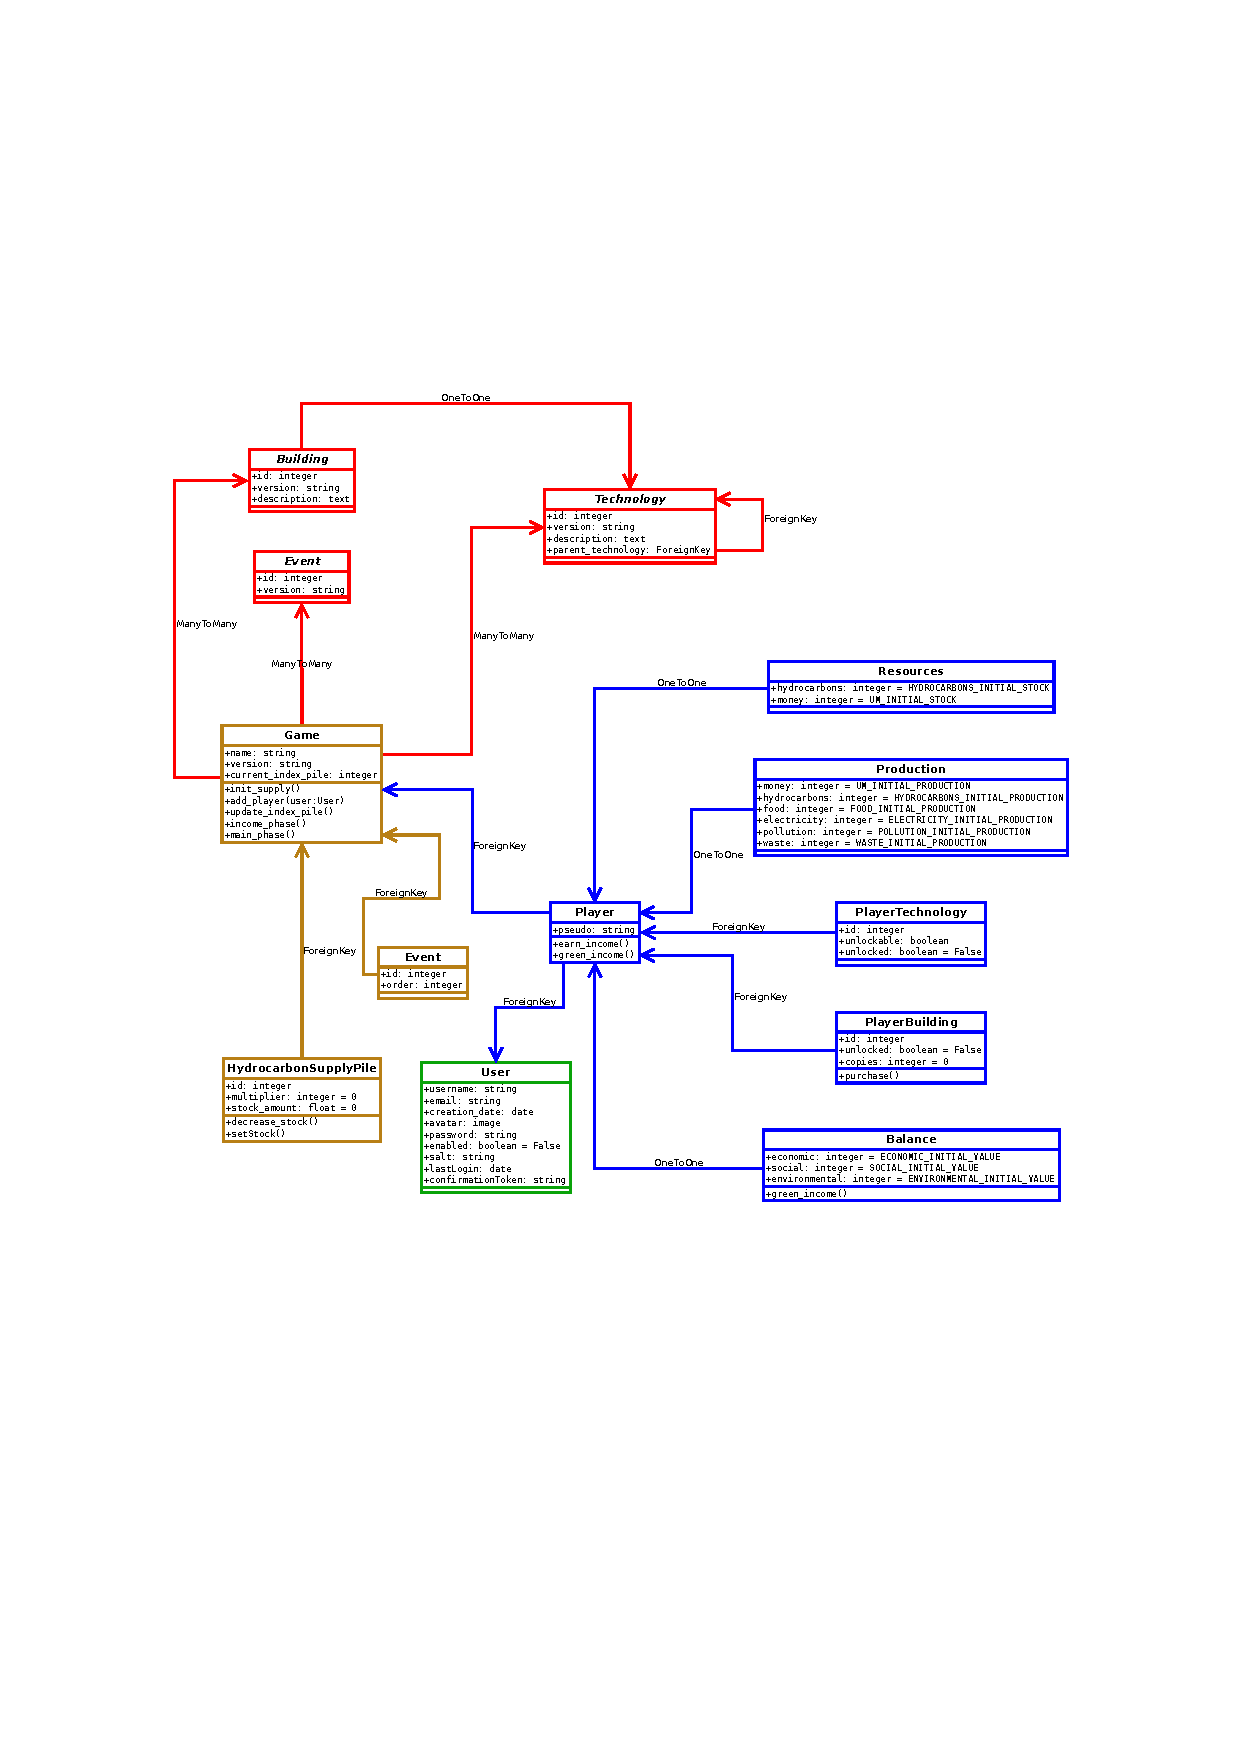
\includegraphics[width=16cm]{../global_uml.pdf}
\caption{Diagramme UML des mod\`eles}
\end{figure}

Comme indiqu\'e sur le diagramme, on a tout d'abord une classe centrale \textbf{Game}, \`a laquelle sont reli\'ees les fixtures (\'ecrites dans des fichiers .json puis charg\'ees en tant qu'instances de mod\`eles) qui d\'ecrivent les instances de \textbf{SourceBuilding} (b\^atiments), \textbf{SourceTechnology} (technologies), et \textbf{SourceEvent} (\'ev\`enements). Puis, \`a \textbf{Game} sont reli\'es avec une relation ForeignKey (many-to-one) les mod\`eles \textbf{HydrocarbonSupplyPile} (piles d'hydrocarbures, qui sont ordonn\'ees par leur index) et \textbf{Event} ("deck" d'\'ev\`enemements pour cette partie, ordonn\'es par leur index, et li\'es en ForeignKey aux \textbf{SourceEvent}). Le deuxi\`eme mod\`ele central de l'architecture du backend est le mod\`ele \textbf{Player} qui est reli\'e \`a \textbf{Game} par une ForeignKey. Chaque \textbf{Player} poss\`ede un \textbf{PlayerState}, auquel sont reli\'es les mod\`eles \textbf{Resources}, \textbf{Production}, \textbf{Balance}, \textbf{Technology}, et \textbf{Building}. De plus, chaque \textbf{Player} est li\'e \`a un \textbf{ShadowPlayer}, qui est lui m\^eme li\'e \`a un \textbf{PlayerState}. Cela permet d'impl\'ementer la pile d'action : au d\'ebut de la phase principale de chaque joueur, on copie le Player dans le ShadowPlayer. Puis, pendant toute la phase les actions effectuée ne modifient que le ShadowPlayer. En cas d'annulation de la pile d'actions, le Player est de nouveau copié dans le ShadowPlayer. Enfin, le Player est mis \`a jour \`a la fin du tour en lui attribuant les nouvelles propriétés du ShadowPlayer.

\subsection{Frontend React}

\subsubsection{Généralités}
Pour programmer le Front-End de notre projet, nous avons choisi d’utiliser la bibliothèque de JavaScript React. React est fondé sur l’usage d’objets appelés composants qui héritent d’une classe « Component » et qui s’organisent selon une structure arborescente. Chaque composant dispose d’un attribut state, qui peut stocker des données nécessaires au composant lui-même et à ses fils, et d’une méthode render, qui retourne un ensemble d’objets HTML et de composants React générés dynamiquement en utilisant des syntaxes JSX à chaque fois que le composant est mis à jour.
Pour les requêtes HTTP assurant la communication entre Front-End et Back-End, nous avons fait usage de la librairie Axios.
Le composant principal qui englobe la totalité des autres s’appelle App et se situe à part dans le fichier du même nom. La méthode render de App peut retourner deux composants différents, Game ou WelcomePage, selon que le joueur est dans une partie ou sur les pages d’accueil.
WelcomePage retourne l’ensemble des composants nécessaires pour se connecter, créer un compte, créer ou rejoindre une partie et qui effectuent les requêtes correspondantes auprès du Back-End. Ces composants sont codés dans le fichier WelcomePage.js auquel est associé le fichier de styles WelcomePage.css.
Game, quant à lui, retourne l’ensemble des composants correspondant à l’interface du jeu en lui-même. Le state de Game contient l’ensemble des données du jeu susceptibles d’évoluer en cours de partie. A quelques rares exceptions près, les calculs concernant la faisabilité des actions par le joueur et la mise à jour des données de la partie sont effectués par le Back-End. Des requêtes HTTP sont déclenchées lors des interactions du joueur avec certains boutons pour garantir les échanges nécessaires avec la base de données. Les composants descendant de Game sont codés dans le fichier Game.js auquel est associé le fichier game.css pour les styles.

\subsubsection{Structure de la page d’accueil}
WelcomePage peut retourner différents composants correspondant aux différentes étapes entre la connexion et le lancement d’une partie. 
En toute logique, le composant retourné en premier est Login qui affiche un formulaire permettant à un joueur ayant déjà un compte de se connecter avec son nom d’utilisateur et son mot de passe. 
Un second composant Signup est accessible depuis Login et affiche un autre formulaire permettant à un joueur n’ayant pas de compte de s’en créer un. 
Si l’un des deux questionnaires est rempli correctement et envoyé, l’utilisateur accède au composant MainMenu qui propose de rejoindre une partie au moyen d’un code ou d’en créer une. 
Finalement, si le joueur choisit de créer une partie, un quatrième composant CreateGame est affiché qui permet au joueur de créer une partie et de se procurer le code de partie correspondant communiqué par le Back-End. Ce code de partie que nous avons déjà évoqué plus haut est nécessaire à d’autres joueurs pour se connecter à la même partie.
Que ce soit par création d’une nouvelle partie ou en en rejoignant une déjà existante, il s’opère un changement dans le composant retourné par App qui devient celui de l’interface du jeu : Game.

\subsubsection{Structure de l’interface du jeu}
Le composant Game peut retourner trois sous-composants différents, chacun correspondant à un onglet de l’interface.
MenuGrid correspond à l’onglet « Menu », sa méthode render retourne des composants affichant les statistiques et ressources du joueur, le menu des actions pouvant être achetées et la file des actions effectuées pendant le tour. 
TechGrid correspond à l’onglet « Technologies » et permet d’afficher le menu des technologies, toujours avec la file des actions du tour.
Finalement, GameInfoPanel devrait, à terme, afficher des statistiques globales du jeu, des évènements et d’autres informations utiles telles que le code de la partie, mais cette page est pour l’instant vide.

\section{El\'ements r\'ealis\'es}

\subsection{Impl\'ementation du backend}

Au niveau du backend, tous les mod\`eles d\'ecrits dans la section pr\'ec\'edente sont impl\'ement\'es. Il manque ainsi l'impl\'ementation des accords d'importation et d'exportation que nous n'avons pas eu le temps de traiter. L'impl\'ementation des int\'eractions entre les mod\`eles existants est compl\`ete. Nous n'avons pas cod\'e tous les b\^atiments et technologies pr\'evues dans les fixtures, mais nous en avons une s\'election repr\'esentative. Certains endpoints de l'API sont op\'erationnels. Ainsi, un visiteur est capable de créer une compte, s'authentifier, créer une partie, en rejoindre une, et lancer une partie. Il manque donc les endpoints servant au d\'eroulement de la partie, que nous n'avons pas eu le temps d'impl\'ementer. Le travail restant pour atteindre une version fonctionnelle du jeu serait cependant une répétition du travail déjà effectué, ce qui ne poserait pas de difficultés supplémentaires.\\
Le système d'authentification retenu repose sur un \'echange de jetons jwt entre le client et le serveur, ce qui permet de contrôler l'accès aux ressources servies par l'API (on souhaite par exemple qu'un joueur donné ne puisse pas accéder aux actions considérées par un autre joueur lors d'un tour). 

\subsection{Impl\'ementation du frontend}

A ce jour, les fonctionnalités du projet qui sont opérationnelles sont la création de compte, la connexion, la création d'une partie et l'accès à une partie déjà créée.
Plus précisément, il est possible à un utilisateur d'accéder au menu principal du projet, soit en s'étant connecté grâce à des identifiants figurant dans la base de données, soit en lui soumettant de nouveaux identifiants associés à une adresse mail. Une fois sur le menu principal, il est possible de créér ou de rejoindre une partie. Le backend est capable de fournir en quelques secondes un token identifiant la partie créée à la demande de l'utilisateur ou bien, un token lui étant donné, de connecter l'utilisateur à une partie en cours. 
Une fois dans l'interface de jeu, les agissements des boutons n'entraînent pour le moment pas d'échanges avec le backend. La fonctionnalité en cours d'implémentation au moment du rendu est la récupération des données du jeu (statistiques des actions et technologies) pour l'affichage. Par ailleurs, les différentes technologies ne disposent pour le moment pas toutes d'images.

\section{Probl\`emes rencontr\'es}

Durant ce projet, nous avons \'et\'es confront\'es \`a plusieurs difficult\'es. Nous avons mis beaucoup de temps \`a mettre un place une API adaptée au projet, en cons\'equence de quoi l'ensemble des liens que nous souhaitions établir entre frontend et backend n'ont pas pu être faits dans les temps. A posteriori, une approche plus progressive et peut-être moins ambitieuse dans laquelle les fonctionnalités élémentaires auraient été implémentées une à une en conservant le lien entre backend et frontend aurait été préférable à celle que nous avons adoptée. Le choix de développer en parallèle les deux parties du projet en visant à obtenir un ensemble de fonctionnalités somme toute assez élaborées s'est avéré contestable, d'autant que les équipes chargées des différentes missions se sont perdues de vue plusieurs fois, rendant les liaisons encore plus difficiles.










\end{document}